%%%%%%%%%%%%%%%%%%%%%%%%%%%%%%%%%%%%%%
% Based on template frmo Nathaniel Johnston
% August 2009
% http://www.nathanieljohnston.com/2009/08/latex-poster-template/
%%%%%%%%%%%%%%%%%%%%%%%%%%%%%%%%%%%%%%

\documentclass[final,plain]{beamer}
\usepackage[size=custom,width=152.4,height=91.44]{beamerposter}
\usepackage{graphicx}			% allows us to import images
\usepackage{palatino}
\usepackage{helvet}
\usepackage{amsmath}
\usepackage{booktabs}
\usepackage{hyperref}

\hypersetup{pdfpagemode=UseNone} % don't show bookmarks on initial view

% added by ss
\renewcommand{\arraystretch}{1.1}
%-----------------------------------------------------------
% Define the column width and poster size
% To set effective sepwid, onecolwid and twocolwid values, first choose how many columns you want and how much separation you want between columns
% The separation I chose is 0.024 and I want 4 columns
% Then set onecolwid to be (1-(4+1)*0.024)/4 = 0.22
% Set twocolwid to be 2*onecolwid + sepwid = 0.464
%-----------------------------------------------------------

\newlength{\sepwid}
\newlength{\onecolwid}
\newlength{\halfcolwid}
\newlength{\twocolwid}
\newlength{\threecolwid}

\setlength{\sepwid}{0.0192\paperwidth}
\setlength{\onecolwid}{0.176\paperwidth}
\setlength{\halfcolwid}{0.0784\paperwidth}
\setlength{\twocolwid}{0.3712\paperwidth}
\setlength{\threecolwid}{0.5664\paperwidth}
\setlength{\topmargin}{-0.5in}
\usetheme{confposter}
\usepackage{exscale}

\newcommand{\bi}{\begin{itemize}}
\newcommand{\ei}{\end{itemize}}
\newcommand{\ttsm}{\tt \small}
\newcommand{\ttfn}{\tt \footnotesize}
\newcommand{\bluebold}{\color{dblue} \bf}
\newcommand{\colonevsep}{\vspace{40mm}}
\newcommand{\coltwovsep}{\vspace{23mm}}
\newcommand{\colthreevsep}{\vspace{12mm}}
\newcommand{\colfourvsep}{\vspace{10mm}}
\newcommand{\colfivevsep}{\vspace{23mm}}

% color for figure legend boxes
\setbeamercolor{legend}{fg=black,bg=mypurple!10}


%-----------------------------------------------------------
% Define colours (see beamerthemeconfposter.sty to change these colour definitions)
%-----------------------------------------------------------

\definecolor{mypurple}{RGB}{88,0,187}

\setbeamercolor{block title}{fg=mypurple,bg=white}
\setbeamercolor{block body}{fg=black,bg=white}
\setbeamercolor{block alerted title}{fg=white,bg=dblue!70}
\setbeamercolor{block alerted body}{fg=black,bg=dblue!10}

%-----------------------------------------------------------
% Name and authors of poster/paper/research
%-----------------------------------------------------------

\title{Data visualizations should be more interactive}
\author{Karl W Broman}

\institute{\normalsize Biostatistics \&
  Medical Informatics, University of Wisconsin--Madison}

%-----------------------------------------------------------
% Start the poster itself
%-----------------------------------------------------------
% The \rmfamily command is used frequently throughout the poster to force a serif font to be used for the body text
% Serif font is better for small text, sans-serif font is better for headers (for readability reasons)
%-----------------------------------------------------------

\begin{document}

\begin{frame}[t]

\begin{columns}[t]
  \begin{column}{\sepwid}\end{column} % empty spacer column

  \begin{column}{\onecolwid}

    \begin{exampleblock}{\Large Abstract}
       {The value of interactive graphics for making sense of
        high-dimensional data has long been appreciated but is still not
        in routine use. Interactive graphics facilitate data exploration,
        are great collaborative tools, allow compressed summary plots to
        be linked to the underlying details, and can be fabulous teaching
        tools. New web-browser-based tools, such as the JavaScript library
        D3, have greatly simplified the development of interactive
        visualizations. A number of R packages, including Shiny and
        rCharts, provide customizable interactive visualizations directly
        from R.  I provide a number of examples to illustrate the
        value of interactive graphics, with live demonstrations on a
        laptop. (I'd initially planned to use
        handheld devices, but the resolution is too poor for what I am
        trying to do.)

     \vspace{18pt}

        \centerline{Live demos:
        \href{http://www.biostat.wisc.edu/~kbroman/posters/ENAR2014}{\tt \textbf{bit.ly/enar2014}}}

     }

    \end{exampleblock}


  \colonevsep % between blocks

    \begin{block}{Opportunities}{

      \bi
      \itemsep18pt
      \item \bluebold Exploration

         \bi \itemsep14pt
         \item Tuning parameters
         \item Identifying outliers
         \item One fancy plot vs 1000 static plots
         \ei

      \item \bluebold Reports for collaborators

         \bi \itemsep14pt
         \item Living documents!
         \item Allow deeper exploration of the results
         \item Cut down on simple questions?
         \ei

      \item \bluebold Big Data

         \bi \itemsep14pt
         \item Don't just rely on summary statistics
         \item Greatly compressed information, but with access to the details
         \item Zoom into dense figures
         \item More exploration, more connections
         \ei

      \item \bluebold Teaching

         \bi \itemsep14pt
         \item Cool things to look at and play with
         \item Animated illustrations of key concepts
         \item Demonstrate data exploration
         \item Enable intro students to explore data
         \ei
      \ei

    }
    \end{block}

  \colonevsep % between blocks


    \begin{block}{Barriers}{
      \bi
      \itemsep18pt
      \item We never learned how
      \item It's a hassle
      \item No consistent platform
      \item Journal articles are static
          \bi
          \item[] (and what else matters?)
          \ei
      \item Most statisticians are still creating terrible static plots
           \bi
           \item[] (even worse, obnoxious tables)
           \ei
      \ei
    }
    \end{block}

  \colonevsep % between blocks


    \begin{block}{But: {\color{mypurple} many} exciting new tools }{
      \bi
      \itemsep18pt
      \item HTML5 + Scalable vector graphics (SVG)
      \item Incredible power of modern web browsers
      \item Javascript-based web tools
      \item \href{http://www.rstudio.com}{RStudio}'s tools
      \ei
    }
    \end{block}

  \end{column}

  \begin{column}{\sepwid} \end{column} % empty spacer column

  \begin{column}{\onecolwid}

    \begin{block}{Options}{

      \bi \itemsep18pt
      \item {\tt \bluebold locator()} and {\tt \bluebold identify()}
      \item {\bluebold ggobi} {\small (\href{http://ggobi.org}{\ttsm ggobi.org})} and
        {\bluebold cranvas}
        {\small (\href{https://github.com/ggobi/cranvas/wiki}{\ttsm github.com/ggobi/cranvas/wiki})}
      \item {\bluebold Mondrian}
        {\small (\href{http://rosuda.org/software/Mondrian/}{\ttsm rosuda.org/software/Mondrian})}
      \item {\bluebold gWidgets}
        {\small (\href{http://gwidgets.r-forge.r-project.org/}{\ttsm gwidgets.r-forge.r-project.org})}
      \item {\bluebold rpanel}
        {\small (\href{http://www.stats.gla.ac.uk/~adrian/rpanel/}{\ttsm www.stats.gla.ac.uk/{\textasciitilde}adrian/rpanel})}
      \item {\bluebold Acinoynx} (aka iPlots eXtreme)
        {\small (\href{http://rforge.net/Acinonyx/}{\ttsm rforge.net/Acinonyx})}
      \item {\bluebold googleVis}
        {\small (\href{https://code.google.com/p/google-motion-charts-with-r/}{\ttsm code.google.com/p/google-motion-charts-with-r})}
      \item {\bluebold gridSVG}
        {\small (\href{http://r-forge.r-project.org/projects/gridsvg/}{\ttsm r-forge.r-project.org/projects/gridsvg})}
      \item {\bluebold RGL}
        {\small (\href{http://rgl.neoscientists.org/}{\ttsm rgl.neoscientists.org})}
      \item \href{http://www.rstudio.com}{RStudio}'s {\tt \bluebold manipulate()} 
        {\small (\href{http://www.rstudio.com/ide/docs/advanced/manipulate}{\ttsm www.rstudio.com/ide/docs/advanced/manipulate})}
      \item \href{http://www.rstudio.com}{RStudio}'s {\bluebold Shiny}
        {\small (\href{http://www.rstudio.com/shiny}{\ttsm www.rstudio.com/shiny})}
      \item \href{http://www.rstudio.com}{RStudio}'s {\bluebold ggvis}
        {\small (\href{http://ggvis.rstudio.com}{\ttsm ggvis.rstudio.com})}
      \item {\bluebold Rcharts}
        {\small (\href{http://rcharts.io}{\ttsm rcharts.io})}
      \item {\bluebold D3} {\small (\href{http://d3js.org}{\ttsm d3js.org})}
      \ei

    }

    \end{block}

  \coltwovsep % between blocks

        \begin{beamercolorbox}[sep=1em, wd=\onecolwid]{legend} \rmfamily

          \centerline{\bluebold \Large simple \quad
            $\longleftrightarrow$ \quad flexible}

           \vspace{48pt}

           \hfill \begin{minipage}{0.3\onecolwid}
            Choose one.

            I choose {\bluebold flexible}.
            \end{minipage}

        \end{beamercolorbox}

  \coltwovsep % between blocks

    \begin{block}{D3}{

       \bi \itemsep18pt
       \item Javascript library for manipulating HTML and SVG elements
       \item Connects data to elements
       \item Low level, but flexible
       \item Used at the \href{http://www.nytimes.com/pages/multimedia/index.html}{NY Times}
       \item I use \href{http://coffeescript.org}{CoffeeScript} rather than JavaScript
       \ei
    }
    \end{block}

  \coltwovsep % between blocks

    \begin{exampleblock}{\Large Summary}
        \bi \itemsep18pt
        \item For high-dimensional data, good visualizations are
          {\color{mypurple} critical}
        \item {\color{mypurple} Interactive} graphics require effort, but they
          \bi
          \item Facilitate exploration
          \item Are great collaborative tools
          \item Enable summaries with access to the details
          \ei
        \item Visualizations must be {\color{mypurple} tailored} to
          the data and questions
        \item {\color{mypurple} D3} is rather low level it
          \bi
          \item Is totally flexible (like R's static graphics)
          \item Provides hours of enjoyment
          \item Can provide other hours of frustration
          \ei
        \ei
    \end{exampleblock}

  \coltwovsep % between blocks

    \begin{block}{Contact}
      \hspace{5em}
        \begin{minipage}{22em}
        \href{http://www.biostat.wisc.edu/~kbroman}{Karl Broman}\\
        {\tt kbroman@biostat.wisc.edu}\\
        \href{http://twitter.com/kwbroman}{\tt @kwbroman} \\
        \href{http://www.biostat.wisc.edu/~kbroman}{\tt www.biostat.wisc.edu/{\textasciitilde}kbroman} \\
        \href{http://github.com/kbroman}{\tt github.com/kbroman}
        \end{minipage}

    \vspace{60pt}
    {\rmfamily \footnotesize
    \centerline{This work was supported in part by NIH grant GM074244.}}
    \end{block}

  \end{column}

\begin{column}{\sepwid} \end{column}                 % empty spacer column

  \begin{column}{\twocolwid}
    \begin{exampleblock}{\Large Example 1: Expression genetics}{
    \begin{center}
    \begin{minipage}[t]{0.6\onecolwid}
    \vspace*{0mm}

    \bi
    \item Mouse intercross, B6 $\times$ BTBR
    \item {\textasciitilde}500 mice
    \item Genotypes at 2057 SNPs
    \ei

    \end{minipage}
    \hspace{0.5\sepwid}
    \begin{minipage}[t]{0.7\onecolwid}
    \vspace*{0mm}

    \bi
    \item Gene expression microarrays in six tissues
    \item Numerous clinical phenotypes
    \ei

    \end{minipage} \end{center}
    }
    \end{exampleblock}

    \vspace{1mm} % between blocks

    \begin{columns}[t]

      \begin{column}{\onecolwid}

        \href{http://www.biostat.wisc.edu/~kbroman/posters/ENAR2014/1a}{
\includegraphics[width=2cm]{Figs/dot1a.pdf}}

        \centerline{\href{http://www.biostat.wisc.edu/~kbroman/posters/ENAR2014/1a}{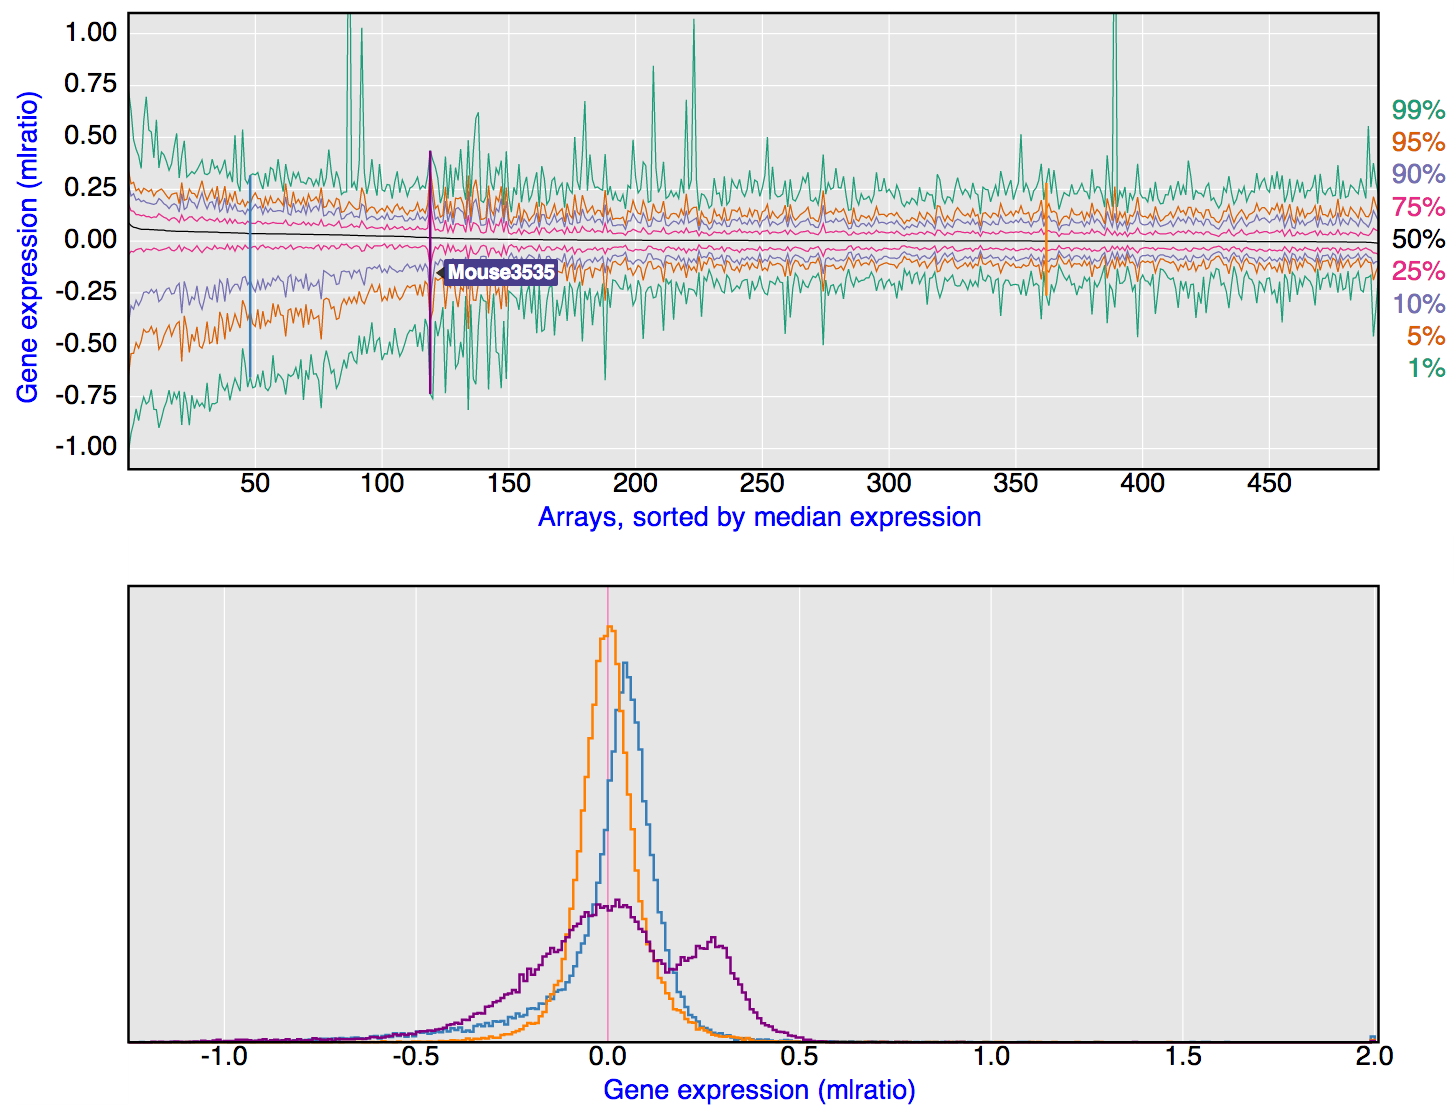
\includegraphics[width=\onecolwid]{Figs/1a.png}}}

      \vspace{10mm} % after legend

        \begin{beamercolorbox}[sep=1em, wd=\onecolwid]{legend} \rmfamily
           These are data from {\textasciitilde}500 gene expression
           microarrays. 

           \vspace{12pt}

           The top panel is like 500 box plots:
           lines are drawn at the 1, 5, \dots, 99 percentiles
           for each of {\textasciitilde}500 distributions. The
           distibutions are sorted by their medians.

           \vspace{12pt}

           If one hovers over a column in the top panel, the corresponding distribution
          is shown below. Click in the top panel for the distribution
          to persist, and click again to make it go away.
        \end{beamercolorbox}


    \colthreevsep % between blocks

        \href{http://www.biostat.wisc.edu/~kbroman/posters/ENAR2014/1b}{
\includegraphics[width=2cm]{Figs/dot1b.pdf}}

        \centerline{\href{http://www.biostat.wisc.edu/~kbroman/posters/ENAR2014/1b}{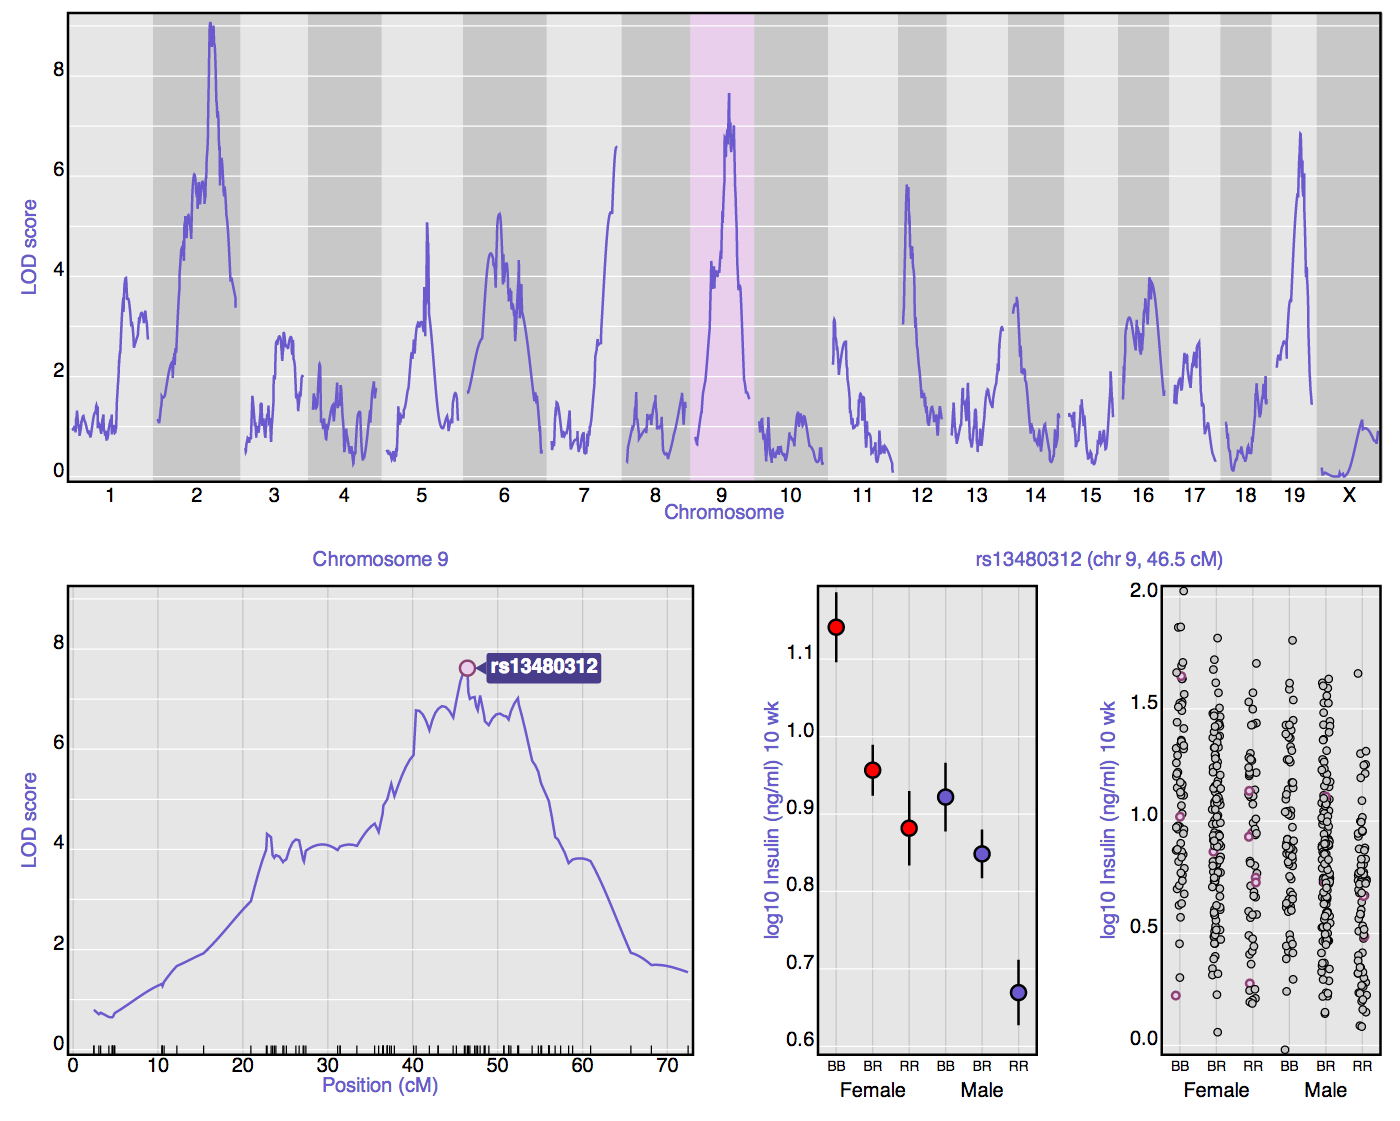
\includegraphics[width=\onecolwid]{Figs/1b.png}}}

      \vspace{10mm} % after legend

        \begin{beamercolorbox}[sep=1em, wd=\onecolwid]{legend} \rmfamily
           A genome scan for genetic loci (called quantitative trait
           loci, QTL) influencing insulin level. The LOD score is a
           log$_{10}$ likelihood ratio measuring the strength of
           association between genotype and phenotype.

           \vspace{12pt}

           Click on a chromosome at the top and a detailed view of the
           LOD curve for that chromosome is shown on the bottom left.
           In the lower-left panel, hover over markers to see names;
           click to view an effect plot and and phenotype-vs-genotype
           plot to the right.
        \end{beamercolorbox}


      \end{column}

      \begin{column}{\sepwid} \end{column} % empty spacer column

      \begin{column}{\onecolwid}

        \href{http://www.biostat.wisc.edu/~kbroman/posters/ENAR2014/1c}{
\includegraphics[width=2cm]{Figs/dot1c.pdf}}

        \centerline{\href{http://www.biostat.wisc.edu/~kbroman/posters/ENAR2014/1c}{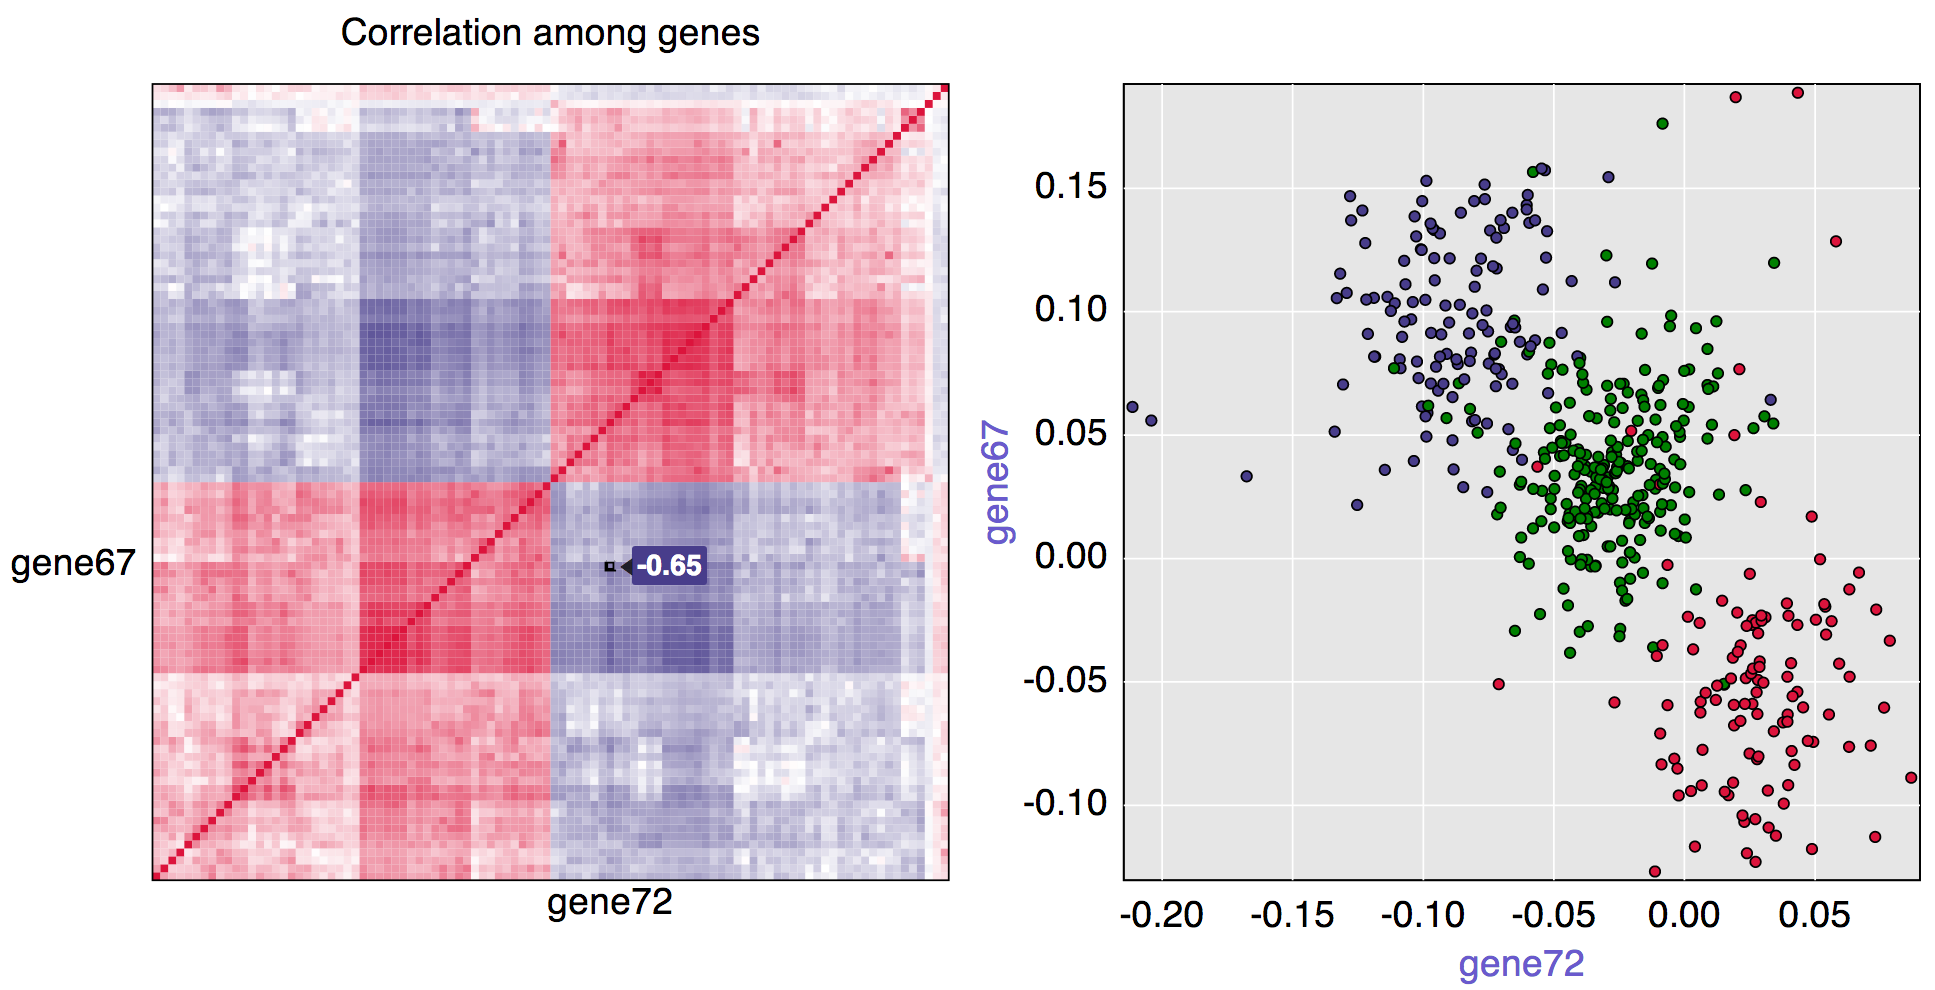
\includegraphics[width=\onecolwid]{Figs/1c.png}}}

      \vspace{10mm} % after legend

        \begin{beamercolorbox}[sep=1em, wd=\onecolwid]{legend} \rmfamily
           Association in gene expression among 100 genes that are
           influenced by a common genetic locus (QTL).  The left panel
           is a heat map of the correlation matrix, with blue = --1
           and red = +1. Hover over pixels in the correlation matrix
           on the left to see the values; click to see the
           corresponding scatterplot on the right. Points in the
           scatterplot are colored by genotype at the underlying QTL.
        \end{beamercolorbox}


    \colfourvsep % between blocks

        \href{http://www.biostat.wisc.edu/~kbroman/posters/ENAR2014/1d}{
\includegraphics[width=2cm]{Figs/dot1d.pdf}}

        \centerline{\href{http://www.biostat.wisc.edu/~kbroman/posters/ENAR2014/1d}{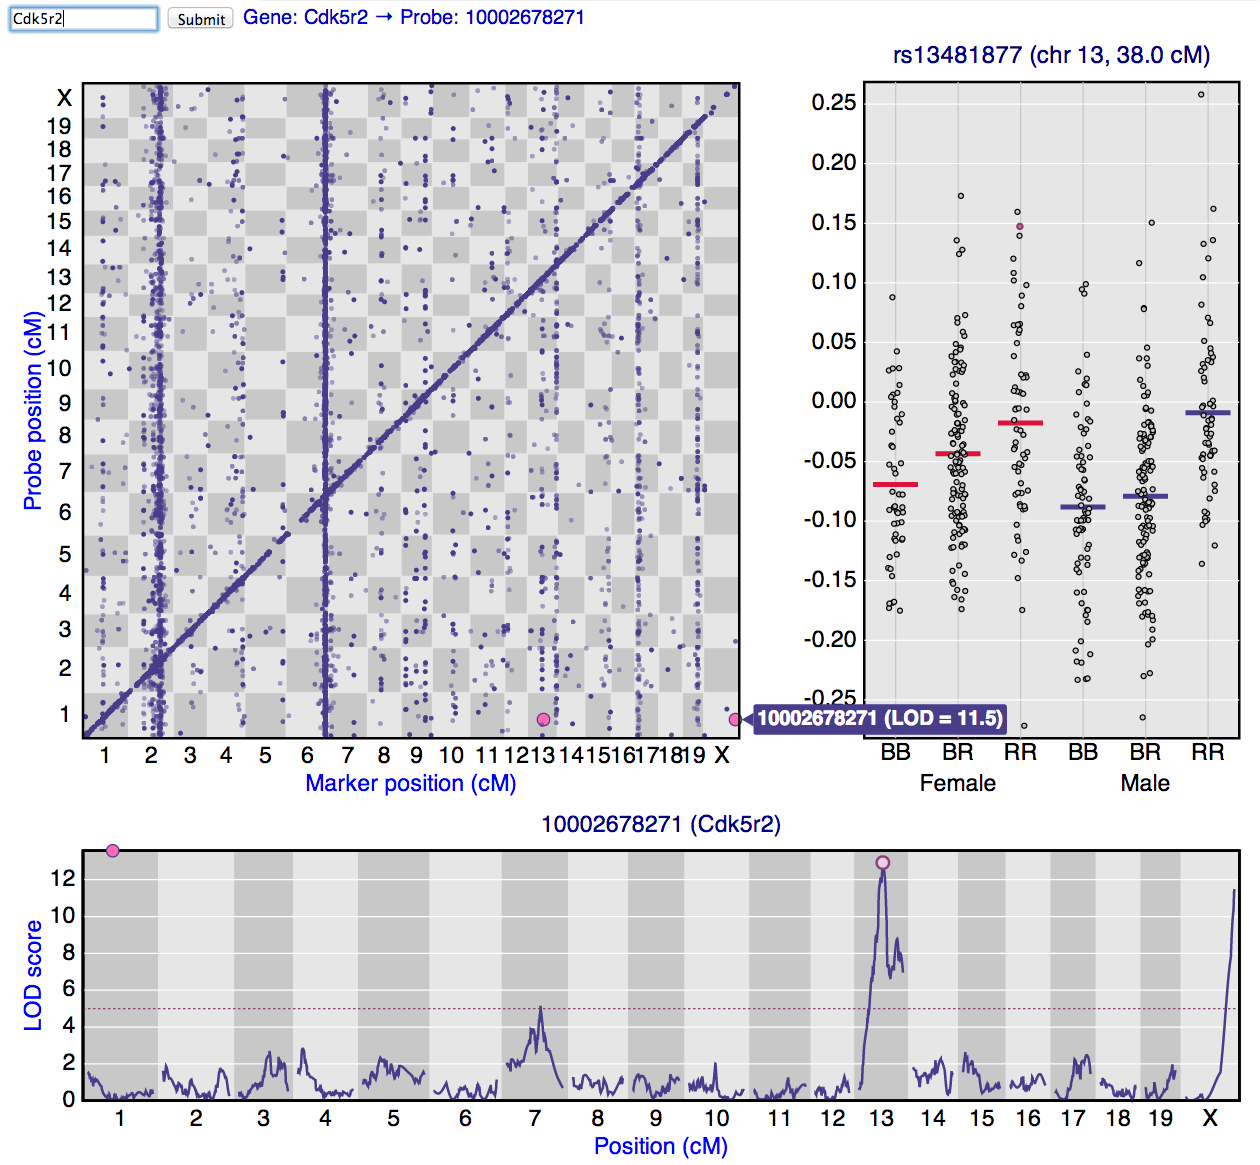
\includegraphics[width=\onecolwid]{Figs/1d.png}}}

      \vspace{10mm} % after legend

        \begin{beamercolorbox}[sep=1em, wd=\onecolwid]{legend} \rmfamily
           An investigation of genetic loci (eQTL) influencing gene
           expression.  In the top-left panel, the x-axis corresponds
           to marker location and the y-axis corresponds to the
           position of probes on a gene expression microarray. Each
           plotted point is an inferred eQTL.

           \vspace{12pt}

           Hover over a point to see the probe ID and LOD score
           (measuring the strength of association); also
           highlighted are any other eQTL for that probe.  Click on
           the point to see the LOD curves below.

           \vspace{12pt}

           Hover over markers in the LOD curve plot to view marker
           names; click on a marker to see the phenotype-vs-genotype
           plot to the right.
        \end{beamercolorbox}


      \end{column}
  \end{columns}
  \end{column}

  \begin{column}{\sepwid} \end{column} % empty spacer column


  \begin{column}{\onecolwid}
    \begin{exampleblock}{\Large Example 2: Gratitropism}{
    \begin{minipage}[t]{\halfcolwid}
    \vspace*{0mm}

    \bi
    \item Response to gravity in Arabidopsis seedlings
    \item Rotate orientation of gravity and video over 8 hrs
    \item Measure the angle of the root tip every 2 min
    \ei

    \end{minipage}
    \hfill
    \begin{minipage}[t]{\halfcolwid}
    \vspace*{0mm}

    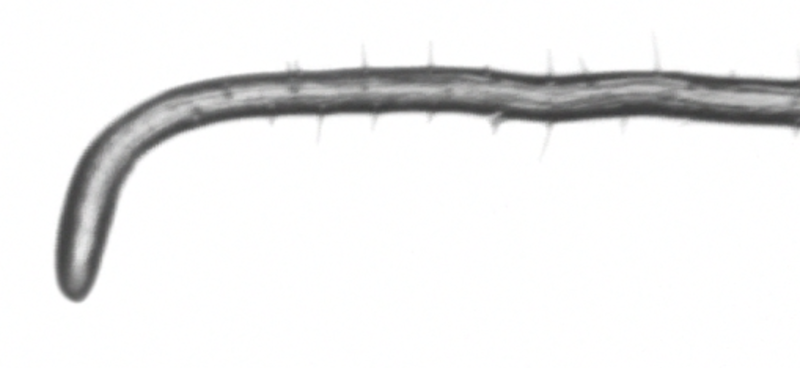
\includegraphics[width=\halfcolwid]{Figs/gravitropism.png}

    \end{minipage} }
    \end{exampleblock}


  \vspace{10mm} % space between blocks

    \href{http://www.biostat.wisc.edu/~kbroman/posters/ENAR2014/2a}{
\includegraphics[width=2cm]{Figs/dot2a.pdf}}

    \centerline{\href{http://www.biostat.wisc.edu/~kbroman/posters/ENAR2014/2a}{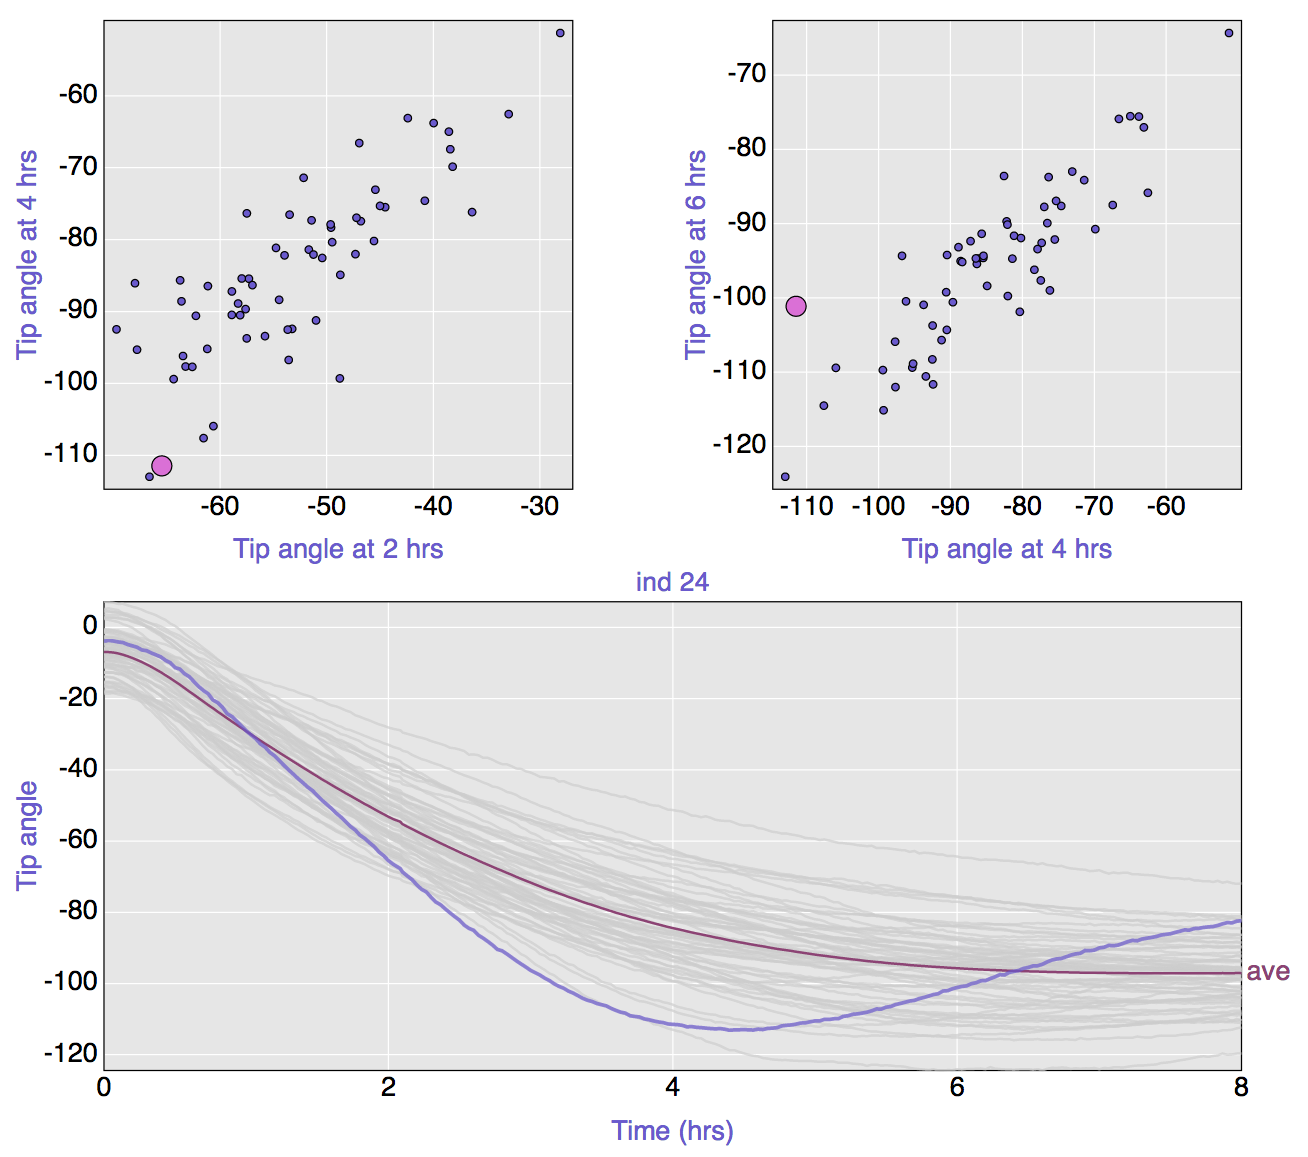
\includegraphics[width=\onecolwid]{Figs/2a.png}}}

      \vspace{10mm} % after legend

        \begin{beamercolorbox}[sep=1em, wd=\onecolwid]{legend} \rmfamily
           Average tip angle over time for 162 Arabidopsis
           lines.

           \vspace{12pt}

          Hover over points in the top panels or curves in the bottom
          panel to highlight the corresponding individual in the other
          panels.
        \end{beamercolorbox}


  \colfivevsep % between blocks

    \href{http://www.biostat.wisc.edu/~kbroman/posters/ENAR2014/2b}{
\includegraphics[width=2cm]{Figs/dot2b.pdf}}

    \centerline{\href{http://www.biostat.wisc.edu/~kbroman/posters/ENAR2014/2b}{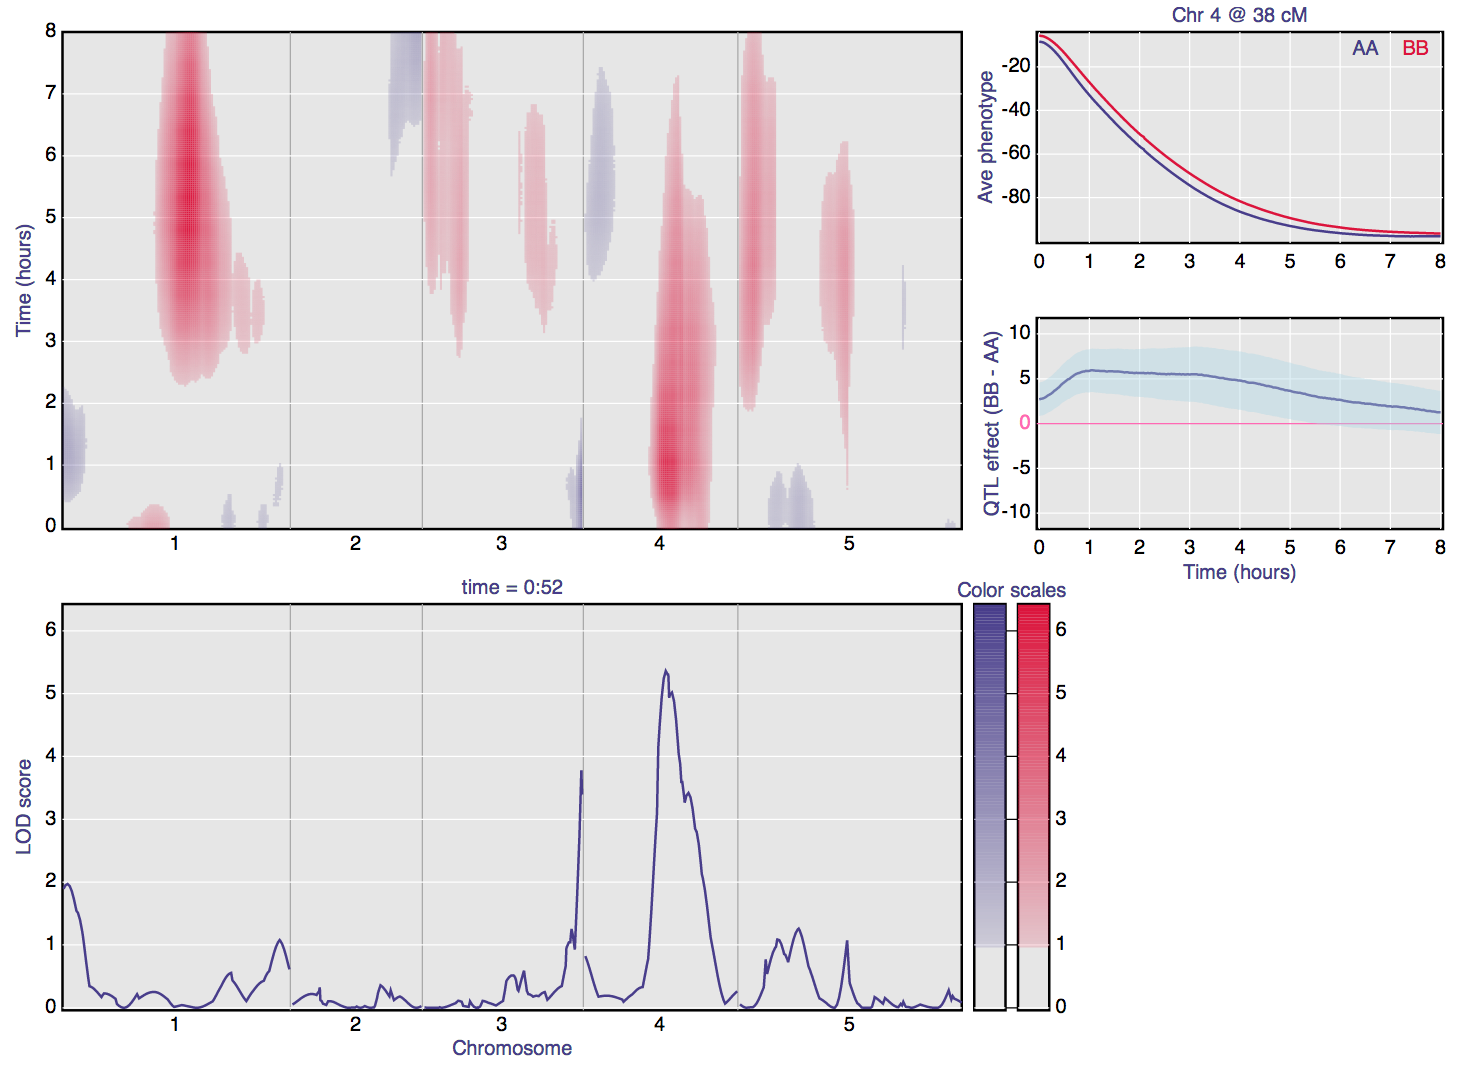
\includegraphics[width=\onecolwid]{Figs/2b.png}}}

      \vspace{10mm} % after legend

        \begin{beamercolorbox}[sep=1em, wd=\onecolwid]{legend} \rmfamily
        The top-left panel is a heat map of a measure association (LOD
        score) between genotype at a fixed position and the phenotype
        at a fixed time.  Red (blue) indicates that BB (AA) lines have larger
        phenotype.
 
        \vspace{12pt}

        When you hover over a point in the top-left plot, the LOD curves for the
        corresponding time are shown below, and the phenotype averages and
        estimated genetic effect (across time) are shown to the right.
        \end{beamercolorbox}


  \end{column}

  \begin{column}{\sepwid}\end{column} % empty spacer column

\end{columns}

%\hrule   % <- uncomment to help check that the columns are the same length

\end{frame}

\end{document}
